\chapter{The Revised Simplex Method and Optimality Conditions}\label{chap:KKT}
\section{The Revised Simplex Method}
Consider an arbitrary linear programming problem, which we will assume is written in standard form:
\begin{equation}
P\left\{
\begin{aligned}
\max\;\; & \mathbf{c}^T\mathbf{x}\\
s.t.\;\; & \mathbf{A}\mathbf{x} = \mathbf{b}\\
& \mathbf{x} \geq \mathbf{0}
\end{aligned}\right.
\end{equation}

The tableau method is a substantially data intensive process as we carry the entire simplex tableau with us as we execute the simplex algorithm. However, consider the data we need at each iteration of the algorithm:
\begin{enumerate}
\item Reduced costs: $\mathbf{c}_\mathbf{B}^T\mathbf{B}^{-1}\mathbf{A}_{\cdot j} - c_j$ for each variable $x_j$ where $j \in \mathcal{J}$ and $\mathcal{J}$ is the set of indices of non-basic variables.

\item Right-hand-side values: $\overline{\mathbf{b}} = \mathbf{B}^{-1}\mathbf{b}$ for use in the minimum ratio test.

\item $\overline{\mathbf{a}}_j = \mathbf{B}^{-1}\mathbf{A}_{\cdot j}$ for use in the minimum ratio test.

\item $\overline{z} = \mathbf{c}_{\mathbf{B}}^T\mathbf{B}^{-1}\mathbf{b}$, the current objective function value. 
\end{enumerate}

The one value that is clearly critical to the computation is $\mathbf{B}^{-1}$ as it appears in each and every computation. It would be far more effective to keep only the values: $\mathbf{B}^{-1}$, $\mathbf{c}_{\mathbf{B}}^T\mathbf{B}^{-1}$, $\overline{\mathbf{b}}$ and $\overline{z}$ and compute the reduced cost values and vectors $\overline{\mathbf{a}}_j$ as we need them. 

Let $\mathbf{w} = \mathbf{c}_\mathbf{B}^{T}\mathbf{B}^{-1}$, then the pertinent information may be stored in a new \textit{revised simplex tableau} with form:
\begin{equation}
\begin{array}{c}
\\
\mathbf{x}_\mathbf{B}
\end{array}
\left[
\begin{array}{c|c}
\mathbf{w} & \overline{z}\\
\hline
\mathbf{B}^{-1} & \overline{\mathbf{b}}
\end{array}\right]
\end{equation}

The revised simplex algorithm is detailed in Algorithm \ref{alg:RevisedSimplex}. 
\begin{algorithm}
\caption{Revised Simplex Algorithm}
\label{alg:RevisedSimplex}
\begin{center}
\begin{minipage}[t]{\textwidth-1em}
\underline{\textbf{Revised Simplex Algorithm}}
\begin{enumerate*}
\item Identify an initial basis matrix $\mathbf{B}$ and compute $\mathbf{B}^{-1}$, $\mathbf{w}$, $\overline{\mathbf{b}}$ and $\overline{z}$ and place these into a revised simplex tableau:
\begin{displaymath}
\begin{array}{c}
\\
\mathbf{x}_\mathbf{B}
\end{array}
\left[
\begin{array}{c|c}
\mathbf{w} & \overline{z}\\
\hline
\mathbf{B}^{-1} & \overline{\mathbf{b}}
\end{array}\right]
\end{displaymath}

\item For each $j \in \mathcal{J}$ use $\mathbf{w}$ to compute: $z_j - c_j = \mathbf{w}\mathbf{A}_{\cdot j} - c_j$. 

\item Choose an entering variable $x_j$ (for a maximization problem, we choose a variable with negative reduced cost, for a minimization problem we choose a variable with positive reduced cost):
\begin{enumerate*}
\item If there is no entering variable, STOP, you are at an optimal solution.
\item Otherwise, continue to Step 4.
\end{enumerate*}

\item Append the column $\overline{\mathbf{a}}_j = \mathbf{B}^{-1}\mathbf{A}_{\cdot j}$ to the revised simplex tableau:
\begin{displaymath}
\begin{array}{c}
\\
\mathbf{x}_\mathbf{B}
\end{array}
\left[
\begin{array}{c|c}
\mathbf{w} & \overline{z}\\
\hline
\mathbf{B}^{-1} & \overline{\mathbf{b}}
\end{array}\right]
\left[
\begin{array}{c}
z_j - c_j\\
\hline
\overline{\mathbf{a}_j}
\end{array}\right]
\end{displaymath}

\item Perform the minimum ratio test and determine a leaving variable (using any leaving variable rule you prefer). 
\begin{enumerate*}
\item If $\overline{\mathbf{a}}_j \leq \mathbf{0}$, STOP, the problem is unbounded.
\item Otherwise, assume that the leaving variable is $x_{B_r}$ which appears in row $r$ of the revised simplex tableau.
\end{enumerate*}

\item Use \textit{row operations} and pivot on the leaving variable row of the column:
\begin{displaymath}
\left[
\begin{array}{c}
z_j - c_j\\
\hline
\overline{\mathbf{a}_j}
\end{array}\right]
\end{displaymath}
transforming the revised simplex tableau into:
\begin{displaymath}
\begin{array}{c}
\\
\mathbf{x}_\mathbf{B}'
\end{array}
\left[
\begin{array}{c|c}
\mathbf{w}' & \overline{z}'\\
\hline
{\mathbf{B}'}^{-1} & \overline{\mathbf{b}}'
\end{array}\right]
\left[
\begin{array}{c}
0\\
\hline
\mathbf{e}_r
\end{array}\right]
\end{displaymath}
where $\mathbf{e}_r$ is an identity column with a 1 in row $r$ (the row that left). The variable $x_j$ is now the $r^\text{th}$ element of $\mathbf{x}_\mathbf{B}$. 

\item Goto Step 2.
\end{enumerate*}
\end{minipage}
\end{center}
\end{algorithm}
In essence, the revised simplex algorithm allows us to avoid computing $\overline{\mathbf{a}}_j$ until we absolutely need to do so. In fact, if we do not apply Dantzig's entering variable rule and simply select the first acceptable entering variable, then we may be able to avoid computing a substantial number of columns in the tableau. 

\begin{example}
Consider a software company who is developing a new program. The company has identified two types of bugs that remain in this software: \textit{non-critical} and \textit{critical}. The company's actuarial firm predicts that the risk associated with these bugs are uniform random variables with mean \$100 per non-critical bug and mean \$1000 per critical bug. The software currently has 50 non-critical bugs and 5 critical bugs.

Assume that it requires 3 hours to fix a non-critical bug and 12 hours to fix a critical bug. For each day (8 hour period) beyond two business weeks (80 hours) that the company fails to ship its product, the actuarial firm estimates it will loose \$500 per day.

We can find the optimal number of bugs of each type the software company should fix assuming it wishes to minimize its exposure to risk using a linear programming formulation. 

Let $x_1$ be the number of non-critical bugs corrected and $x_2$ be the number of critical software bugs corrected. Define:
\begin{gather}
y_1 = 50 - x_1\\
y_2 = 5 - x_2
\end{gather}
Here $y_1$ is the number of non-critical bugs that are not fixed while $y_2$ is the number of critical bugs that are not fixed.

The time (in hours) it takes to fix these bugs is:
\begin{equation}
3x_1 + 12x_2
\end{equation}
Let:
\begin{equation}
y_3 = \frac{1}{8}\left(80 - 3x_1 - 12x_2\right)
\end{equation}
Then $y_3$ is a variable that is unrestricted in sign and determines the amount of time (in days) either over or under the two-week period that is required to ship the software. As an unrestricted variable, we can break it into two components:
\begin{equation}
y_3 = z_1 - z_2
\end{equation}
We will assume that $z_1, z_2 \geq 0$. If $y_3 > 0$, then $z_1 > 0$ and $z_2 = 0$. In this case, the software is completed ahead of the two-week deadline. If $y_3 < 0$, then $z_1 = 0$ and $z_2 > 0$. In this case the software is finished after the two-week deadline. Finally, if $y_3 = 0$, then $z_1 = z_2 = 0$ and the software is finished precisely on time. 

We can form the objective function as:
\begin{equation}
z = 100y_1 + 1000y_2 + 500z_2
\end{equation}
The linear programming problem is then:
\begin{equation}
\begin{aligned}
\min\;\;z = & y_1 + 10y_2 + 5z_2\\
s.t.\;\;& x_1 + y_1 = 50\\
		& x_2 + y_2 = 5\\
		& \frac{3}{8}x_1 + \frac{3}{2}x_2 + z_1 - z_2 = 10\\
		& x_1, x_2, y_1, y_2, z_1, z_2 \geq 0
\end{aligned}
\end{equation}
Notice we have modified the objective function by dividing by 100. This will make the arithmetic of the simplex algorithm easier. The matrix of coefficients for this problem is:
\begin{equation}
\begin{bmatrix}
x_1 & x_2 & y_1 & y_2 & z_1 & z_2\\
\hline 
1 	& 0   	 & 1 & 0 & 0 & 0\\
0 	& 1   	 & 0 & 1 & 0 & 0\\
\frac{3}{8} & \frac{3}{2} & 0 & 0 & 1 & -1
\end{bmatrix}
\end{equation}
Notice there is an identity matrix embedded inside the matrix of coefficients. Thus a good initial basic feasible solution is $\{y_1, y_2, z_1\}$. The initial basis matrix is $\mathbf{I}_3$ and naturally, 
$\mathbf{B}^{-1} = \mathbf{I}_3$ as a result. We can see that $\mathbf{c_B} = [1\; 10\; 0]^T$. It follows that $\mathbf{c}_\mathbf{B}^T\mathbf{B}^{-1} = \mathbf{w} = [1\; 10\; 0]$.

Our initial revised simplex tableau is thus:
\begin{equation}
\begin{array}{c}
z\\
y_1\\
y_2\\
z_1
\end{array}
\left[
\begin{array}{ccc|c}
1	&	10	&	0	&	100\\
\hline
1	&	0	&	0	&	50\\
0	&	1	&	0	&	5\\
0	&	0	&	1	&	10
\end{array}
\right]
\end{equation}
There are three variables that might enter at this point, $x_1$, $x_2$ and $z_1$. We can compute the reduced costs for each of these variables using the columns of the $\mathbf{A}$ matrix, the coefficients of these variables in the objective function and the current $\mathbf{w}$ vector (in row 0 of the revised simplex tableau). We obtain:
\begin{gather*}
z_1 - c_1 = \mathbf{w}\mathbf{A}_{\cdot 1} - c_1 = 
	\begin{bmatrix}1&10&0\end{bmatrix}
	\begin{bmatrix}1\\0\\3/8\end{bmatrix} - 0 = 1\\
z_2 - c_2 = \mathbf{w}\mathbf{A}_{\cdot 2} - c_2 = 
	\begin{bmatrix}1&10&0\end{bmatrix}
	\begin{bmatrix}0\\1\\3/2\end{bmatrix} - 0 = 10\\
z_6 - c_6 = \mathbf{w}\mathbf{A}_{\cdot 6} - c_6 = 
	\begin{bmatrix}1&10&0\end{bmatrix}
	\begin{bmatrix}0\\0\\-1\end{bmatrix} - 5 = -5
\end{gather*}
By Dantzig's rule, we enter variable $x_2$. We append $\mathbf{B}^{-1}\mathbf{A}_{\cdot 2}$ and the reduced cost to the revised simplex tableau to obtain:
\begin{equation}
\begin{array}{c}
z\\
y_1\\
y_2\\
z_1
\end{array}
\left[
\begin{array}{ccc|c}
1	&	10	&	0	&	100\\
\hline
1	&	0	&	0	&	50\\
0	&	1	&	0	&	5\\
0	&	0	&	1	&	10
\end{array}
\right]
\left[
\begin{array}{c}
10\\
\hline
0\\
\fbox{1}\\
3/2
\end{array}
\right]
\begin{array}{c}
MRT\\
-\\
5\\
20/3
\end{array}
\end{equation}
After pivoting on the indicated element, we obtain the new tableau:
\begin{equation}
\begin{array}{c}
z\\
y_1\\
x_2\\
z_1
\end{array}
\left[
\begin{array}{ccc|c}
1	&	0	&	0	&	50\\
\hline
1	&	0	&	0	&	50\\
0	&	1	&	0	&	5\\
0	&	-3/2	&	1	&	5/2
\end{array}
\right]
\end{equation}
We can compute reduced costs for the non-basic variables (except for $y_2$, which we know will \textbf{not} re-enter the basis on this iteration) to obtain:
\begin{gather*}
z_1 - c_1 = \mathbf{w}\mathbf{A}_{\cdot 1} - c_1 = 1\\
z_6 - c_6 = \mathbf{w}\mathbf{A}_{\cdot 6} - c_6 = -5
\end{gather*}
In this case, $x_1$ will enter the basis and we augment our revised simplex tableau to obtain:
\begin{equation}
\begin{array}{c}
z\\
y_1\\
x_2\\
z_1
\end{array}
\left[
\begin{array}{ccc|c}
1	&	0	&	0	&	50\\
\hline
1	&	0	&	0	&	50\\
0	&	1	&	0	&	5\\
0	&	-3/2	&	1	&	5/2
\end{array}
\right]
\left[
\begin{array}{c}
1\\
\hline
1\\
0\\
3/8
\end{array}
\right]
\begin{array}{c}
MRT\\
50\\
-\\
\fbox{20/3}
\end{array}
\end{equation}
Note that:
\begin{displaymath}
\mathbf{B}^{-1}\mathbf{A}_{\cdot 1} = 
\begin{bmatrix}
1 & 0 & 0\\
0 & 1 & 0\\
0 & -3/2 & 1
\end{bmatrix}
\begin{bmatrix}
1\\0\\3/8
\end{bmatrix} = 
\begin{bmatrix}
1\\0\\3/8
\end{bmatrix}
\end{displaymath}
This is the $\bar{\mathbf{a}}_1$ column that is appended to the right hand side of the tableau along with $z_1 - c_1 = 1$. After pivoting, the tableau becomes:
\begin{equation}
\begin{array}{c}
z\\
y_1\\
x_2\\
x_1
\end{array}
\left[
\begin{array}{ccc|c}
1	&	4	&	-8/3	&	130/3\\
\hline
1	&	4	&	-8/3	&	130/3\\
0	&	1	&	0	&	5\\
0	&	-4	&	8/3	&	20/3
\end{array}
\right]
\end{equation}
We can now check our reduced costs. Clearly, $z_1$ will not re-enter the basis. Therefore, we need only examine the reduced costs for the variables $y_2$ and $z_2$.
\begin{gather*}
z_4 - c_4 = \mathbf{w}\mathbf{A}_{\cdot 4} - c_4 = -6\\
z_6 - c_6 = \mathbf{w}\mathbf{A}_{\cdot 6} - c_6 = -7/3
\end{gather*}
Since all reduced costs are now negative, no further minimization is possible and we conclude we have arrived at an optimal solution.

Two things are interesting to note: first, the solution for the number of non-critical software bugs to fix is non-integer. Thus, in reality the company must fix either 6 or 7 of the non-critical software bugs. The second thing to note is that this economic model helps to explain why some companies are content to release software that contains known bugs. In making a choice between releasing a flawless product or making a quicker (larger) profit, a selfish, profit maximizer will always choose to fix only those bugs it must fix and release sooner rather than later. 
\end{example}

\begin{exercise} Solve the following problem using the revised simplex algorithm.
\begin{displaymath}
\begin{aligned}
\max\;\;&x_1 + x_2\\
s.t.\;\;&2x_1 + x_2 \leq 4\\
&x_1 + 2x_2 \leq 6\\
&x_1, x_2 \geq 0
\end{aligned}
\end{displaymath}
\label{exer:RevisedSimplex}
\end{exercise}

\section{Farkas' Lemma and Theorems of the Alternative}
\begin{lemma}[Farkas' Lemma] Let $\mathbf{A} \in \mathbb{R}^{m \times n}$ and $\mathbf{c} \in \mathbb{R}^n$ be a row vector. Suppose $\mathbf{x} \in \mathbb{R}^n$ is a column vector and $\mathbf{w} \in \mathbb{R}^m$ is a row vector. Then exactly one of the following systems of inequalities has a solution:
\begin{enumerate}
\item $\mathbf{A}\mathbf{x} \geq \mathbf{0}$ and $\mathbf{c}\mathbf{x} < 0$ \textit{or}
\item $\mathbf{w}\mathbf{A} = \mathbf{c}$ and $\mathbf{w} \geq \mathbf{0}$
\end{enumerate}
\label{lem:Farkas}
\end{lemma}
\begin{remark} Before proceeding to the proof, it is helpful to restate the lemma in the following way:
\begin{enumerate}
\item 
\textit{If there is a vector $\mathbf{x} \in \mathbb{R}^n$ so that $\mathbf{A}\mathbf{x} \geq \mathbf{0}$ and $\mathbf{c}\mathbf{x} < 0$, then there \textbf{is no} vector $\mathbf{w} \in \mathbb{R}^m$ so that $\mathbf{w}\mathbf{A} = \mathbf{c}$ and $\mathbf{w} \geq \mathbf{0}$. }

\vspace*{1em}
\item
\textit{Conversely, if there is a vector $\mathbf{w} \in \mathbb{R}^m$ so that $\mathbf{w}\mathbf{A} = \mathbf{c}$ and $\mathbf{w} \geq \mathbf{0}$, then there \textbf{is no} vector $\mathbf{x} \in \mathbb{R}^n$ so that $\mathbf{A}\mathbf{x} \geq \mathbf{0}$ and $\mathbf{c}\mathbf{x} < 0$.}
\end{enumerate}
\end{remark}

\begin{proof} We can prove Farkas' Lemma using the fact that a bounded linear programming problem has an extreme point solution. Suppose that System 1 has a solution $\mathbf{x}$. If System 2 also has a solution $\mathbf{w}$, then 
\begin{equation}
\mathbf{w}\mathbf{A} = \mathbf{c} \implies \mathbf{w}\mathbf{A}\mathbf{x} = \mathbf{c}\mathbf{x}.
\end{equation}
The fact that System 1 has a solution ensures that $\mathbf{cx} < 0$ and therefore $\mathbf{w}\mathbf{A}\mathbf{x} < 0$. However, it also ensures that $\mathbf{Ax} \geq \mathbf{0}$. The fact that System 2 has a solution implies that $\mathbf{w} \geq \mathbf{0}$. Therefore we must conclude that:
\begin{equation}
\mathbf{w} \geq \mathbf{0} \text{ and } \mathbf{Ax} \geq \mathbf{0} \implies \mathbf{w}\mathbf{A}\mathbf{x} \geq \mathbf{0}.
\end{equation}
This contradiction implies that if System 1 has a solution, then System 2 cannot have a solution.

Now, suppose that System 1 has no solution. We will construct a solution for System 2. If System 1 has no solution, then there is no vector $\mathbf{x}$ so that $\mathbf{cx} < 0$ and $\mathbf{Ax} \geq \mathbf{0}$. Consider the linear programming problem:
\begin{equation}
P_F\left\{
\begin{aligned}
\min\;\; & \mathbf{cx}\\
s.t.\;\; & \mathbf{Ax} \geq \mathbf{0}
\end{aligned}\right.
\end{equation} 
Clearly $\mathbf{x} = \mathbf{0}$ is a feasible solution to this linear programming problem and furthermore is optimal. To see this, note that the fact that there is no $\mathbf{x}$ so that $\mathbf{cx} < 0$ and $\mathbf{Ax} \geq \mathbf{0}$, it follows that $\mathbf{cx} \geq 0$; i.e., $0$ is a lower bound for the linear programming problem $P_F$. At $\mathbf{x} = \mathbf{0}$, the objective achieves its lower bound and therefore this must be an optimal solution. Therefore $P_F$ is bounded and feasible.

We can covert $P_F$ to standard form through the following steps: 
\begin{enumerate}
\item Introduce two new vectors $\mathbf{y}$ and $\mathbf{z}$ with $\mathbf{y},\mathbf{z} \geq \mathbf{0}$ and write $\mathbf{x} = \mathbf{y} - \mathbf{z}$ (since $\mathbf{x}$ is unrestricted).
\item Append a vector of surplus variables $\mathbf{s}$ to the constraints. 
\end{enumerate}
This yields the new problem:
\begin{equation}
P_F'\left\{
\begin{aligned}
\min\;\; & \mathbf{cy}-\mathbf{cz}\\
s.t.\;\; & \mathbf{Ay} - \mathbf{A}\mathbf{z} - \mathbf{I}_m\mathbf{s} = \mathbf{0}\\
& \mathbf{y}, \mathbf{z}, \mathbf{s} \geq \mathbf{0}
\end{aligned}\right.
\end{equation} 

Applying Theorems \ref{thm:EPSoln} and \ref{thm:BFSEP}, we see we can obtain an optimal basic feasible solution for Problem $P_F'$ in which the reduced costs for the variables are all negative (that is, $z_j - c_j \leq 0$ for $j=1,\dots,2n+m$). Here we have $n$ variables in vector $\mathbf{y}$, $n$ variables in vector $\mathbf{z}$ and $m$ variables in vector $\mathbf{s}$. Let $\mathbf{B} \in \mathbb{R}^{m \times m}$ be the basis matrix at this optimal feasible solution with basic cost vector $\mathbf{c}_\mathbf{B}$. Let $\mathbf{w} = \mathbf{c}_\mathbf{B}\mathbf{B}^{-1}$ (as it was defined for the revised simplex algorithm). 

Consider the columns of the simplex tableau corresponding to a variable $x_k$ (in our original $\mathbf{x}$ vector). The variable $x_k = y_k - z_k$. Thus, these two columns are additive inverses. That is, the column for $y_k$ will be $\mathbf{B}^{-1} \mathbf{A}_{\cdot k}$, while the column for $z_k$ will be $\mathbf{B}^{-1} (-\mathbf{A}_{\cdot k}) = -\mathbf{B}^{-1} \mathbf{A}_{\cdot k}$. Furthermore, the objective function coefficient will be precisely opposite as well. Thus the fact that $z_j - c_j \leq 0$ for all variables implies that:
\begin{gather*}
\mathbf{w}\mathbf{A}_{\cdot k} - c_k \leq 0 \text{ \textbf{and} }\\
-\mathbf{w}\mathbf{A}_{\cdot k} + c_k \leq 0 \text{ \textbf{and} }\\
\end{gather*}
That is, we obtain
\begin{equation}
\mathbf{w}\mathbf{A} = \mathbf{c}
\end{equation}
since this holds for all columns of $\mathbf{A}$. 

Consider the surplus variable $s_k$. Surplus variables have zero as their coefficient in the objective function. Further, their simplex tableau column is simply $\mathbf{B}^{-1}(-\mathbf{e}_k) = -\mathbf{B}^{-1}\mathbf{e}_k$. The fact that the reduced cost of this variable is non-positive implies that:
\begin{equation}
\mathbf{w}(-\mathbf{e}_k) - 0 = -\mathbf{w}\mathbf{e}_k \leq 0
\end{equation}
Since this holds for all surplus variable columns, we see that $-\mathbf{w} \leq \mathbf{0}$ which implies $\mathbf{w} \geq \mathbf{0}$. Thus, the optimal basic feasible solution to Problem $P_F'$ must yield a vector $\mathbf{w}$ that solves System 2. 

Lastly, the fact that if System 2 does not have a solution, then System 1 does follows from contrapositive on the previous fact we just proved. 
\end{proof}
\begin{exercise} Suppose we have two statements $A$ and $B$ so that:
\begin{gather*}
A \equiv \text{System 1 has a solution.}\\
B \equiv \text{System 2 has a solution.}
\end{gather*}
Our proof showed explicitly that $\text{NOT } A \implies B$. Recall that contrapositive is the logical rule that asserts that:
\begin{equation}
X \implies Y \equiv \text{NOT }Y \implies \text{NOT }X
\end{equation}
Use contrapositive to prove explicitly that if System 2 has no solution, then System 1 must have a solution. [Hint: $\text{NOT }\text{NOT }X \equiv X$.]
\end{exercise}

\subsection{Geometry of Farkas' Lemma}
Farkas' Lemma has a pleasant geometric interpretation\footnote{Thanks to Akinwale Akinbiyi for pointing out a typo in this discussion.}. Consider System 2: namely:
\begin{displaymath}
\mathbf{w}\mathbf{A} = \mathbf{c}\text{ \textbf{and} } \mathbf{w} \geq \mathbf{0}
\end{displaymath}
Geometrically, this states that $\mathbf{c}$ is inside the positive cone generated by the \textit{rows of} $\mathbf{A}$. That is, let $\mathbf{w} = (w_1,\dots,w_m)$. Then we have:
\begin{equation}
w_1 \mathbf{A}_{1\cdot} + \dots + w_m \mathbf{A}_{m\cdot}
\end{equation}
and $w_i \geq 0$ for $i=1,\dots,m$. Thus $\mathbf{c}$ is a positive combination of the rows of $\mathbf{A}$. 
This is illustrated in Figure \ref{fig:System2}.
\begin{figure}[htbp]
\centering
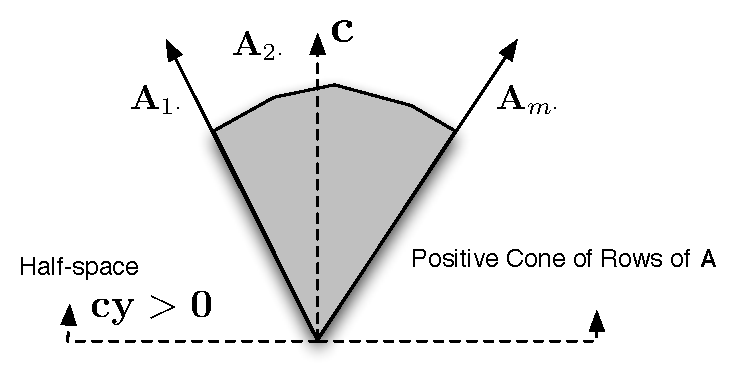
\includegraphics[scale=0.75]{System2.pdf}
\caption{System 2 has a solution if (and only if) the vector $\mathbf{c}$ is contained inside the positive cone constructed from the rows of $\mathbf{A}$. }
\label{fig:System2}
\end{figure}
On the other hand, suppose System 1 has a solution. Then let $\mathbf{y} = -\mathbf{x}$. System 1 states that $\mathbf{A}\mathbf{y} \leq \mathbf{0}$ and $\mathbf{c}\mathbf{y} > 0$. That means that each row of $\mathbf{A}$ (as a vector) must be at a right angle or obtuse to $\mathbf{y}$. (Since $\mathbf{A}_{i \cdot}\mathbf{x} \geq \mathbf{0}$.) Further, we know that the vector $\mathbf{y}$ must be acute with respect to the vector $\mathbf{c}$. This means that System 1 has a solution only if the vector $\mathbf{c}$ is not in the positive cone of the rows of $\mathbf{A}$ or equivalently the intersection of the open half-space $\{\mathbf{y} : \mathbf{c}\mathbf{y} > 0\}$ and the set of vectors $\{\mathbf{y} : \mathbf{A}_{i\cdot}\mathbf{y} \leq \mathbf{0}, i=1,\dots m\}$ is non-empty. This set is the cone of vectors perpendicular to the rows of $\mathbf{A}$. This is illustrated in Figure \ref{fig:System1}
\begin{figure}[htbp]
\centering
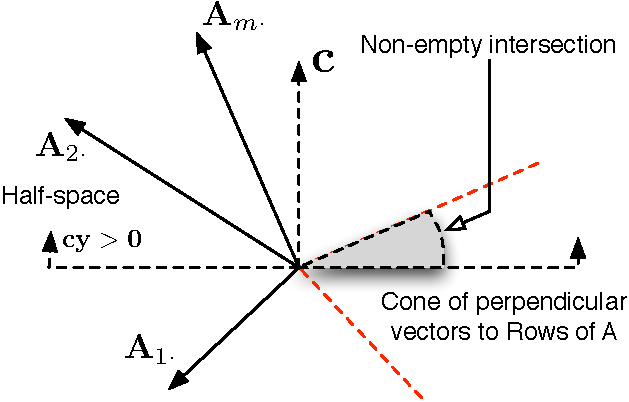
\includegraphics[scale=0.75]{System1.pdf}
\caption{System 1 has a solution if (and only if) the vector $\mathbf{c}$ is not contained inside the positive cone constructed from the rows of $\mathbf{A}$.}
\label{fig:System1}
\end{figure}
\begin{example} Consider the matrix:
\begin{displaymath}
\mathbf{A} = \begin{bmatrix}
1 & 0\\
0 & 1
\end{bmatrix}
\end{displaymath}
and the vector $\mathbf{c} = \begin{bmatrix}1 & 2\end{bmatrix}$. Then clearly, we can see that the vector $\mathbf{w} = \begin{bmatrix}1 & 2\end{bmatrix}$ will satisfy System 2 of Farkas' Lemma, since $\mathbf{w} \geq \mathbf{0}$ and $\mathbf{w}\mathbf{A} = \mathbf{c}$. 

Contrast this with $\mathbf{c}' = \begin{bmatrix}1 & -1\end{bmatrix}$. In this case, we can choose $\mathbf{x} = \begin{bmatrix}0 & 1\end{bmatrix}^T$. Then $\mathbf{A}\mathbf{x} = \begin{bmatrix}0 & 1\end{bmatrix}^T \geq \mathbf{0}$ and $\mathbf{c}'\mathbf{x} = -1$. Thus $\mathbf{x}$ satisfies System 1 of Farkas' Lemma.

These two facts are illustrated in Figure \ref{fig:FarkasExample}. Here, we see that $\mathbf{c}$ is inside the positive cone formed by the rows of $\mathbf{A}$, while $\mathbf{c}'$ is not. 
\begin{figure}[ht]
\centering
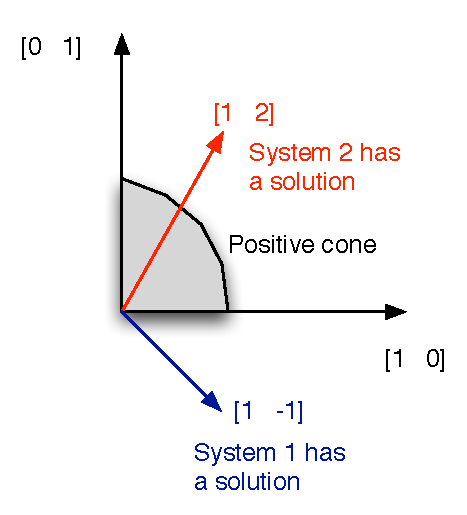
\includegraphics[scale=0.5]{ExampleFarkas.pdf}
\caption{An example of Farkas' Lemma: The vector $\mathbf{c}$ is inside the positive cone formed by the rows of $\mathbf{A}$, but $\mathbf{c}'$ is not.}
\label{fig:FarkasExample} 
\end{figure}
\end{example}

\begin{exercise} Consider the following matrix: 
\begin{displaymath}
\mathbf{A} = \begin{bmatrix}
1 & 0\\
1 & 1
\end{bmatrix}
\end{displaymath}
and the vector $\mathbf{c} = \begin{bmatrix}1 & 2\end{bmatrix}$. For this matrix and this vector, does System 1 have a solution or does System 2 have a solution? [Hint: Draw a picture illustrating the positive cone formed by the rows of $\mathbf{A}$. Draw in $\mathbf{c}$. Is $\mathbf{c}$ in the cone or not?]
\end{exercise}

\subsection{Theorems of the Alternative}
Farkas' lemma can be manipulated in many ways to produce several equivalent statements. The collection of all such theorems are called \textit{Theorems of the Alternative} and are used \textit{extensively} in optimization theory in proving optimality conditions. We state two that will be useful to us.

\begin{corollary} Let $\mathbf{A} \in \mathbb{R}^{k \times n}$ and $\mathbf{E} \in \mathbb{R}^{l \times n}$.  Let $\mathbf{c} \in \mathbb{R}^n$ be a row vector. Suppose $\mathbf{d} \in \mathbb{R}^n$ is a column vector and $\mathbf{w} \in \mathbb{R}^k$ is a row vector and $\mathbf{v} \in \mathbf{R}^{l}$ is a row vector.  Let:
\begin{displaymath}
\mathbf{M} = \begin{bmatrix}
\mathbf{A}\\
\mathbf{E}
\end{bmatrix}
\end{displaymath}
and
\begin{displaymath}
\mathbf{u} = \begin{bmatrix}
\mathbf{w} & \mathbf{v}
\end{bmatrix}
\end{displaymath}
Then exactly one of the following systems has a solution:
\begin{enumerate}
\item $\mathbf{M}\mathbf{d} \leq \mathbf{0}$ and $\mathbf{c}\mathbf{d} > 0$ \textit{or}
\item $\mathbf{u}\mathbf{M} = \mathbf{c}$ and $\mathbf{u}\geq \mathbf{0}$
\end{enumerate}
\label{cor:KKT}
\end{corollary}
\begin{proof} Let $\mathbf{x} = -\mathbf{d}$. Then $\mathbf{M}\mathbf{d} \leq \mathbf{0}$ implies $\mathbf{M}\mathbf{x} \geq \mathbf{0}$ and $\mathbf{c}\mathbf{d} > 0$ implies $\mathbf{c}\mathbf{x} < 0$. This converts System 1 to the System 1 of Farkas' Lemma. System 2 is already in the form found in Farkas' Lemma. This completes the proof. 
\end{proof}

%\begin{exercise} Proof the following corollary to Farkas' Lemma: Let $\mathbf{A} \in \mathbb{R}^{m \times n}$ and $\mathbf{c} \in \mathbb{R}^n$ be a row vector. Suppose $\mathbf{y} \in \mathbb{R}^n$ is a column vector and $\mathbf{w} \in \mathbb{R}^m$ is a row vector. Exactly one of the following two systems has a solution:
%\begin{enumerate}
%\item $\mathbf{A}\mathbf{y} \leq \mathbf{0}$, $\mathbf{y} \leq \mathbf{0}$ and $\mathbf{c}\mathbf{y} > 0$
%\item $\mathbf{w}\mathbf{A}\leq \mathbf{c}$ and $\mathbf{w}\geq \mathbf{0}$
%\end{enumerate}
%[Hint: This is an example in the \cite{BJS04}.]
%\end{exercise}
\begin{exercise} Prove the following corollary to Farkas' Lemma:
\begin{corollary} Let $\mathbf{A} \in \mathbb{R}^{m \times n}$ and $\mathbf{c} \in \mathbb{R}^n$ be a row vector. Suppose $\mathbf{d} \in \mathbb{R}^n$ is a column vector and $\mathbf{w} \in \mathbb{R}^m$ is a row vector and $\mathbf{v} \in \mathbf{R}^{n}$ is a row vector. Then exactly one of the following systems of inequalities has a solution:
\begin{enumerate}
\item $\mathbf{A}\mathbf{d} \leq \mathbf{0}$, $\mathbf{d} \geq \mathbf{0}$ and $\mathbf{c}\mathbf{d} > 0$ \textit{or}
\item $\mathbf{w}\mathbf{A} - \mathbf{v} = \mathbf{c}$ and $\mathbf{w}, \mathbf{v} \geq \mathbf{0}$
\end{enumerate}
\end{corollary}
[Hint: Write System 2 from this corollary as $\mathbf{w}\mathbf{A} - \mathbf{I}_n \mathbf{v} = \mathbf{c}$ and then re-write the system with an augmented vector $[\mathbf{w}\;\;\;\mathbf{v}]$ with an appropriate augmented matrix. Let $\mathbf{M}$ be the augmented matrix you identified. Now write System 1 from Farkas' Lemma using $\mathbf{M}$ and $\mathbf{x}$. Let $\mathbf{d} = -\mathbf{x}$ and expand System 1 until you obtain System 1 for this problem.]
%\begin{proof} Our objective is to transform these systems into something that looks like the systems of Farkas' Lemma. Consider System 2. We may write the equality as:
%\begin{equation}
%\mathbf{w}\mathbf{A} - \mathbf{I}_n \mathbf{v} = \mathbf{c} \iff 
%\begin{bmatrix}\mathbf{w} & \mathbf{v}\end{bmatrix}\begin{bmatrix}\mathbf{A}\\-\mathbf{I}_n\end{bmatrix} = \mathbf{c}
%\end{equation} 
%Define:
%\begin{gather*}
%\mathbf{z} = \begin{bmatrix}\mathbf{w} & \mathbf{v}\end{bmatrix}\\
%\mathbf{M} = \begin{bmatrix}\mathbf{A}\\-\mathbf{I}_n\end{bmatrix}
%\end{gather*}
%Then System 2 is equivalent to: $\mathbf{z}\mathbf{M} = \mathbf{c}$ and $\mathbf{z} \geq \mathbf{0}$. We can now apply Farkas' Lemma to this system. In that case, System 1 becomes: $\mathbf{M}\mathbf{x} \geq \mathbf{0}$ and $\mathbf{c}\mathbf{x} < 0$. For $\mathbf{x} \in \mathbb{R}^{n}$. 
%
%Apply the definition of $\mathbf{M}$ we have:
%\begin{equation}
%\mathbf{M}\mathbf{x} \geq \mathbf{0} \iff \begin{bmatrix}\mathbf{A}\\-\mathbf{I}_n\end{bmatrix}\mathbf{x} \geq \mathbf{0}
%\end{equation}
%The previous equation implies the following system of inequalities:
%\begin{gather}
%\mathbf{A}\mathbf{x} \geq \mathbf{0}\\
%-\mathbf{I}_n\mathbf{x} \geq \mathbf{0}
%\end{gather}
%Let $\mathbf{d} = -\mathbf{x}$. Then we have:
%\begin{displaymath}
%\begin{aligned}
%&\mathbf{A}(-\mathbf{d}) \geq \mathbf{0} \iff \mathbf{A}\mathbf{d} \leq \mathbf{0}\\
%&-\mathbf{I}_n(-\mathbf{d}) \geq \mathbf{0} \iff \mathbf{I}_n\mathbf{d} \geq \mathbf{0} \iff \mathbf{d} \geq \mathbf{0}
%\end{aligned}
%\end{displaymath}
%Lastly, $\mathbf{c}\mathbf{x} < 0$ becomes $\mathbf{c}(-\mathbf{d}) < 0$ or $\mathbf{c}\mathbf{d} > 0$. 
%
%Thus we have shown (by Farkas' Lemma) that either System 1 or System 2 has a solution. This completes the proof.
%\end{proof}
\end{exercise}

\section{The Karush-Kuhn-Tucker Conditions}
\begin{theorem} Consider the linear programming problem:
\begin{equation}
P\left\{
\begin{aligned}
\max\;\; & \mathbf{c}\mathbf{x}\\
s.t.\;\; & \mathbf{A}\mathbf{x} \leq \mathbf{b}\\
& \mathbf{x} \geq \mathbf{0}
\end{aligned}\right.
\end{equation}
with $\mathbf{A} \in \mathbb{R}^{m \times n}$, $\mathbf{b} \in \mathbb{R}^m$ and (row vector) $\mathbf{c} \in \mathbb{R}^n$. Then $\mathbf{x}^* \in \mathbb{R}^n$ is an optimal solution\footnote{Thanks to Rich Benjamin for pointing out the fact I was missing ``\dots is an optimal solution\dots''} to $P$ if and only if there exists (row) vectors $\mathbf{w}^* \in \mathbb{R}^m$ and $\mathbf{v}^* \in \mathbb{R}^n$ so that:
\begin{align}
\text{Primal Feasibility}&\left\{ 
\begin{aligned}
\mathbf{A}\mathbf{x}^* \leq \mathbf{b}\\
\mathbf{x}^* \geq \mathbf{0}
\end{aligned}\right.\\
\text{Dual Feasibility}&\left\{ 
\begin{aligned}
\mathbf{w}^*\mathbf{A} - \mathbf{v}^* = \mathbf{c}\\
\mathbf{w}^* \geq \mathbf{0}\\
\mathbf{v}^* \geq \mathbf{0}
\end{aligned}\right.\\
\text{Complementary Slackness}&\left\{ 
\begin{aligned}
\mathbf{w}^*\left(\mathbf{A}\mathbf{x}^* - \mathbf{b}\right) = 0\\
\mathbf{v}^*\mathbf{x}^* = 0
\end{aligned}\right.
\end{align}
\label{thm:KKT}
\end{theorem}
\begin{remark} The vectors $\mathbf{w}^*$ and $\mathbf{v}^*$ are sometimes called \textit{dual variables} for reasons that will be clear in the next chapter. They are also sometimes called \textit{Lagrange Multipliers}. You may have encountered Lagrange Multipliers in your Math 230 or Math 231 class. These are the same kind of variables except applied to linear optimization problems. 
There is one element in the dual variable vector $\mathbf{w}^*$ for each constraint of the form $\mathbf{A}\mathbf{x} \leq \mathbf{b}$ and one element in the dual variable vector $\mathbf{v}^*$ for each constraint of the form $\mathbf{x} \geq \mathbf{0}$. 
\end{remark}
\begin{proof} Suppose that $\mathbf{x}^*$ is an optimal solution to Problem $P$. Consider only the \textit{binding constraints} at $\mathbf{x}^*$. For simplicity, write the constraints $\mathbf{x} \geq \mathbf{0}$ as $-\mathbf{x} \leq \mathbf{0}$. Then we can form a new system of equations of the form:
\begin{align}
\begin{bmatrix} \mathbf{A}_E \\ \mathbf{E} \end{bmatrix} \mathbf{x} = \mathbf{b}_E
\end{align}
where $\mathbf{E}$ is a matrix of negative identity matrix rows corresponding to the variables $x_k$ that are equal to zero. That is, if $x_k = 0$, then $-x_k = 0$ and the negative identity matrix row $-\mathbf{e}^T_k$ will appear in $\mathbf{E}$ where $-\mathbf{e}^T_k \in \mathbb{R}^{1 \times n}$. Here $\mathbf{b}_\mathbf{E}$ are the right hand sides of the binding constraints. Let:
\begin{displaymath}
\mathbf{M} = \begin{bmatrix}
\mathbf{A}_E\\
\mathbf{E}
\end{bmatrix}
\end{displaymath}
The fact that $\mathbf{x}^*$ is optimal implies that there is no improving direction $\mathbf{d}$ at the point $\mathbf{x}^*$. That is, there is no $\mathbf{d}$ so that $\mathbf{M}\mathbf{d} \leq \mathbf{0}$ and $\mathbf{c}^T\mathbf{d} > 0$. Otherwise, by moving in this direction we could find a new point $\hat{\mathbf{x}} = \mathbf{x}^* + \lambda\mathbf{d}$ (with $\lambda$ sufficiently small) so that:
\begin{displaymath}
\mathbf{M}\hat{\mathbf{x}} = \mathbf{M}\mathbf{x}^* + \lambda \mathbf{M}\mathbf{d} \leq \mathbf{b}_E
\end{displaymath}
The (negative) identity rows in $\mathbf{E}$ ensure that $\hat{\mathbf{x}} \geq \mathbf{0}$. 
It follows that:
\begin{displaymath}
\mathbf{c}\hat{\mathbf{x}} = \mathbf{c}^T\left( \mathbf{x}^* + \lambda\mathbf{d}\right) = \mathbf{c}\mathbf{x}^* + \lambda\mathbf{c}\mathbf{d} > \mathbf{c}\mathbf{x}^*
\end{displaymath}
That is, this point is both feasible and has a larger objective function value than $\mathbf{x}^*$. 

We can now apply Corollary \ref{cor:KKT} to show that there are vectors $\mathbf{w}$ and $\mathbf{v}$ so that:
\begin{align}
\begin{bmatrix}\mathbf{w} & \mathbf{v}\end{bmatrix}
\begin{bmatrix}
\mathbf{A}_E \\
\mathbf{E}\label{eqn:DualFeas1}
\end{bmatrix} = \mathbf{c}\\
\mathbf{w} \geq \mathbf{0}\\
\mathbf{v} \geq \mathbf{0}
\end{align}

Let $I$ be the indices of the rows of $\mathbf{A}$ making up $\mathbf{A}_E$ and let $J$ be the indices of the variables that are zero (i.e., binding in $\mathbf{x} \geq \mathbf{0}$). Then we can re-write Equation \ref{eqn:DualFeas1} as:
\begin{equation}
\sum_{i \in I} w_i \mathbf{A}_{i\cdot} - \sum_{j \in J} v_j \mathbf{e}_j = \mathbf{c}
\label{eqn:ConversePart}
\end{equation}
The vector $\mathbf{w}$ has dimension equal to the number of binding constraints of the form $\mathbf{A}_{i\cdot}\mathbf{x} = \mathbf{b}$ while the vector $\mathbf{v}$ has dimension equal to the number of binding constraints of the form $\mathbf{x} \geq \mathbf{0}$. We can extend $\mathbf{w}$ to $\mathbf{w}^*$ by adding $0$ elements for the constraints where $\mathbf{A}_{i\cdot}\mathbf{x} < \mathbf{b}_i$. Similarly we can extend $\mathbf{v}$ to $\mathbf{v}^*$ by adding $0$ elements for the constraints where $x_j > 0$. The result is that:
\begin{align}
\mathbf{w}^*\left(\mathbf{A}\mathbf{x}^* - \mathbf{b}\right) = 0\\
\mathbf{v}^*\mathbf{x}^* = 0
\end{align}
In doing this we maintain $\mathbf{w}^*,\mathbf{v}^* \geq \mathbf{0}$ and simultaneously guarantee that $\mathbf{w}^* \mathbf{A} - \mathbf{v}^* = \mathbf{c}$. 

To prove the converse we assume that the KKT conditions hold and we are given vectors $\mathbf{x}^*$, $\mathbf{w}^*$ and $\mathbf{v}^*$. We will show that $\mathbf{x}^*$ solves the linear programming problem. By dual feasibility, we know that Equation \ref{eqn:ConversePart} holds with $\mathbf{w} \geq \mathbf{0}$ and $\mathbf{v} \geq \mathbf{0}$ defined as before and the given point $\mathbf{x}^*$. Let $\mathbf{x}$ be an alternative point. 
We can multiply both side of Equation \ref{eqn:ConversePart} by $(\mathbf{x}^* - \mathbf{x})$. This leads to:
\begin{equation}
\left\{\sum_{i \in I} w_i \mathbf{A}_{i\cdot}\mathbf{x}^* - \sum_{j \in J} v_j \mathbf{e}_j\mathbf{x}^*\right\}- 
\left\{\sum_{i \in I} w_i \mathbf{A}_{i\cdot}\mathbf{x} - \sum_{j \in J} v_j \mathbf{e}_j\mathbf{x}^* \right\} = \mathbf{c}\mathbf{x}^* - \mathbf{c}\mathbf{x}
\label{eqn:KKTMiddle}
\end{equation}
We know that $\mathbf{A}_{i\cdot}\mathbf{x}^* = \mathbf{b}_i$ for $i \in I$ and that $x^*_j = 0$ for $j \in J$. We can use this to simplify Equation \ref{eqn:KKTMiddle}:
\begin{equation}
\sum_{i \in I} w_i \left(\mathbf{b}_i - \mathbf{A}_{i\cdot}\mathbf{x}\right) + \sum_{j \in J} v_j \mathbf{e}_j\mathbf{x} = \mathbf{c}\mathbf{x}^* - \mathbf{c}\mathbf{x}
\end{equation}
The left hand side must be non-negative, since $\mathbf{w} \geq \mathbf{0}$ and $\mathbf{v} \geq \mathbf{0}$, $b_i - \mathbf{A}_{i\cdot}\mathbf{x} \geq 0$ for all $i$, and $\mathbf{x} \geq 0$ and thus it follows that $\mathbf{x}^*$ must be an optimal point since $\mathbf{c}\mathbf{x}^* - \mathbf{c}\mathbf{x} \geq 0$. This completes the proof.
\end{proof}
\begin{remark} The expressions:
\begin{align}
\text{Primal Feasibility}&\left\{ 
\begin{aligned}
\mathbf{A}\mathbf{x}^* \leq \mathbf{b}\\
\mathbf{x}^* \geq \mathbf{0}
\end{aligned}\right.\\
\text{Dual Feasibility}&\left\{ 
\begin{aligned}
\mathbf{w}^*\mathbf{A} - \mathbf{v}^* = \mathbf{c}\\
\mathbf{w}^* \geq \mathbf{0}\\
\mathbf{v}^* \geq \mathbf{0}
\end{aligned}\right.\\
\text{Complementary Slackness}&\left\{ 
\begin{aligned}
\mathbf{w}^*\left(\mathbf{A}\mathbf{x}^* - \mathbf{b}\right) = 0\\
\mathbf{v}^*\mathbf{x}^* = 0
\end{aligned}\right.
\end{align}
are called the \textit{Karush-Kuhn-Tucker (KKT) conditions} of optimality. Note there is one element in $\mathbf{w}$ for each row of the constraints $\mathbf{A}\mathbf{x} \leq \mathbf{b}$ and one element in the vector $\mathbf{v}$ for each constraint of the form $\mathbf{x} \geq \mathbf{0}$. The vectors $\mathbf{w}$ and $\mathbf{v}$ are sometimes called \textit{dual variables} and sometimes called Lagrange Multipliers.

We can think of dual feasibility as expressing the following interesting fact: at optimality, the gradient of the objective function $\mathbf{c}$ can be expressed as a positive combination of the gradients of the binding constraints written as less-than-or-equal-to inequalities. That is, the gradient of the constraint $\mathbf{A}_{i\cdot}\mathbf{x} \leq \mathbf{b}_i$ is $\mathbf{A}_{i\cdot}$ and the gradient of the constraint $-{x}_j \leq 0$ is $-\mathbf{e}_j$. More specifically, the vector $\mathbf{c}$ is in the \textit{cone} generated by the binding constraints at optimality. 
\end{remark}

\begin{example}
Consider the Toy Maker Problem (Equation \ref{eqn:ToyMakerEx}) with Dual Variables (Lagrange Multipliers) listed next to their corresponding constraints:
\begin{displaymath}
\left\{
\begin{aligned}
\max\;\;& z(x_1,x_2) = 7x_1 + 6x_2 & \quad \text{\textbf{Dual Variable}}\\
s.t.\;\;&  3x_1 + x_2 \leq 120 & \quad (w_1)\\
& x_1 + 2x_2 \leq 160 & \quad (w_1)\\
& x_1 \leq 35 & \quad (w_3)\\
& x_1 \geq 0 & \quad (v_1)\\
& x_2 \geq 0 & \quad (v_2)
\end{aligned}
\right.
\end{displaymath}
In this problem we have:
\begin{displaymath}
\mathbf{A} = \begin{bmatrix}
3 & 1\\
1 & 2 \\
1 & 0
\end{bmatrix}\quad \mathbf{b} = \begin{bmatrix}120\\160\\35\end{bmatrix} \quad
\mathbf{c} = \begin{bmatrix}7 & 6\end{bmatrix}
\end{displaymath}
Then the KKT conditions can be written as:
\begin{displaymath}
\text{Primal Feasibility}\left\{
\begin{aligned}
& \begin{bmatrix}
3 & 1\\
1 & 2 \\
1 & 0
\end{bmatrix}\begin{bmatrix}x_1\\x_2\end{bmatrix} \leq \begin{bmatrix}120\\160\\35\end{bmatrix}\\
& \begin{bmatrix}x_1\\x_2\end{bmatrix} \geq \begin{bmatrix}0\\0\end{bmatrix}
\end{aligned}\right.
\end{displaymath}
\begin{displaymath}
\text{Dual Feasibility}\left\{
\begin{aligned}
& \begin{bmatrix}w_1&w_2&w_3\end{bmatrix}\begin{bmatrix}
3 & 1\\
1 & 2 \\
1 & 0
\end{bmatrix} - \begin{bmatrix}v_1 & v_2\end{bmatrix} = \begin{bmatrix}7 & 6\end{bmatrix}\\
& \begin{bmatrix}w_1&w_2&w_3\end{bmatrix} \geq \begin{bmatrix}0&0&0\end{bmatrix}\\
& \begin{bmatrix}v_1&v_2\end{bmatrix} \geq \begin{bmatrix}0&0\end{bmatrix}
\end{aligned}\right.
\end{displaymath}
\begin{displaymath}
\text{Complementary Slackness}\left\{
\begin{aligned}
& \begin{bmatrix}w_1&w_2&w_3\end{bmatrix}\left( \begin{bmatrix}
3 & 1\\
1 & 2 \\
1 & 0
\end{bmatrix}\begin{bmatrix}x_1\\x_2\end{bmatrix} \leq \begin{bmatrix}120\\160\\35\end{bmatrix} - \begin{bmatrix}120\\160\\35\end{bmatrix}\right)\\
& \begin{bmatrix}v_1&v_2\end{bmatrix} \begin{bmatrix}x_1&x_2\end{bmatrix} = 0
\end{aligned}\right.
\end{displaymath}
Recall that at optimality, we had $x_1 = 16$ and $x_2 = 72$. The binding constraints in this case where 
\begin{gather*}
3x_1 + x_2 \leq 120\\
x_1 + 2x_2 \leq 160
\end{gather*}
To see this note that if $3(16)+72 = 120$ and $16+2(72) = 160$. Then we should be able to express $\mathbf{c} = [7\;\;\;6]$ (the vector of coefficients of the objective function) as a positive combination of the gradients of the binding constraints:
\begin{gather*}
\nabla(7x_1 + 6x_2) = \begin{bmatrix}7 & 6\end{bmatrix}\\
\nabla(3x_1 + x_2) = \begin{bmatrix}3 & 1\end{bmatrix}\\
\nabla(x_1 + 2x_2) = \begin{bmatrix}1 & 2\end{bmatrix}
\end{gather*}
That is, we wish to solve the linear equation:
\begin{equation}
\begin{bmatrix}w_1 & w_2\end{bmatrix}\begin{bmatrix}3 & 1\\1 & 2\end{bmatrix} = \begin{bmatrix}7 & 6\end{bmatrix}
\end{equation}
Note, this is how Equation \ref{eqn:ConversePart} looks when we apply it to this problem. The result is a system of equations:
\begin{gather*}
3w_1 + w_2 = 7\\
w_1 + 2w_2 = 6
\end{gather*}
A solution to this system is $w_1 = \frac{8}{5}$ and $w_2 =\frac{11}{5}$. This fact is illustrated in Figure \ref{fig:GradientCone}. 

Figure \ref{fig:GradientCone} shows the gradient cone formed by the binding constraints at the optimal point for the toy maker problem. 
\begin{figure}[htbp]
\centering
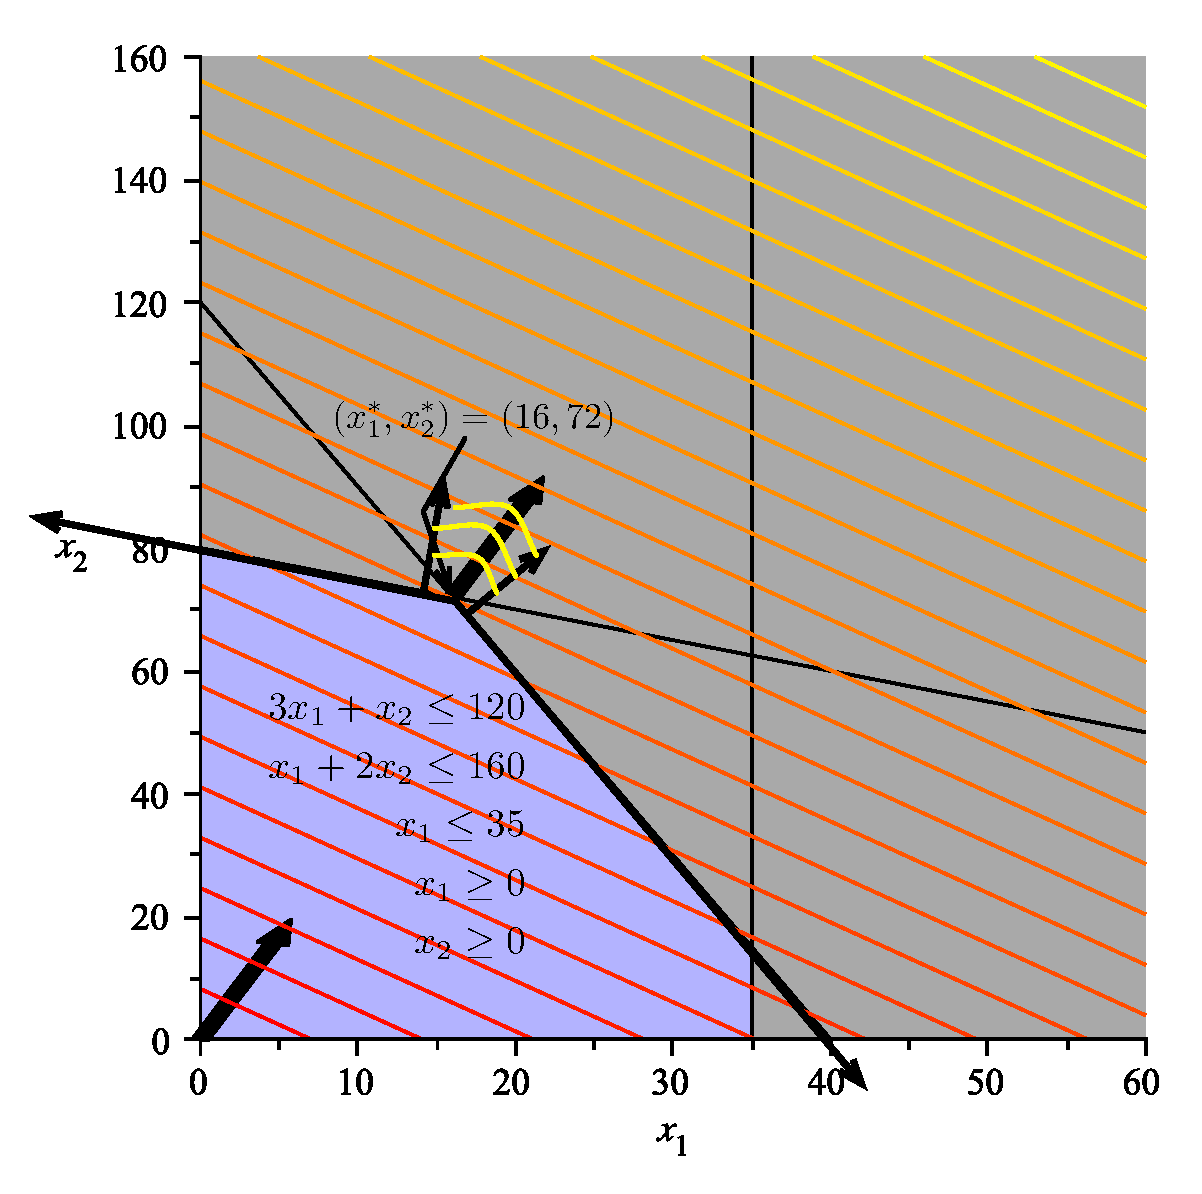
\includegraphics[scale=0.35]{GradientCone.pdf}
\caption{The Gradient Cone: At optimality, the cost vector $\mathbf{c}$ is obtuse with respect to the directions formed by the binding constraints. It is also contained inside the cone of the gradients of the binding constraints, which we will discuss at length later.}
\label{fig:GradientCone}
\end{figure}
Since $x_1, x_2 > 0$, we must have $v_1 = v_2 = 0$. Moreover, since $x_1 < 35$, we know that $x_1 \leq 35$ is not a binding constraint and thus its dual variable $w_3$ is also zero. This leads to the conclusion:
\begin{displaymath}
\begin{bmatrix}
x_1^*\\
x_2^*
\end{bmatrix} = \begin{bmatrix}
16\\
72
\end{bmatrix} \quad 
\begin{bmatrix}
w_1^* & w_2^* & w_3^*
\end{bmatrix} = \begin{bmatrix}8/5 & 11/5 & 0\end{bmatrix} \quad \begin{bmatrix} v_1^* & v_2^*\end{bmatrix} = \begin{bmatrix}0 & 0\end{bmatrix}
\end{displaymath}
and the KKT conditions are satisfied.
\end{example}

\begin{exercise} Consider the problem:
\begin{displaymath}
\begin{aligned}
\max\;\;&x_1 + x_2\\
s.t.\;\;&2x_1 + x_2 \leq 4\\
&x_1 + 2x_2 \leq 6\\
&x_1, x_2 \geq 0
\end{aligned}
\end{displaymath}
Write the KKT conditions for an optimal point for this problem. (You will have a vector $\mathbf{w} = [w_1 \;\;\; w_2]$ and a vector $\mathbf{v} = [v_1\;\;\;v_2]$). 

Draw the feasible region of the problem. At the optimal point you identified in Exercise \ref{exer:RevisedSimplex}, identify the binding constraints and draw their gradients. Show that the objective function is in the positive cone of the gradients of the binding constraints at this point. (Specifically find $\mathbf{w}$ and $\mathbf{v}$.)
\label{exer:FindKKT}
\end{exercise}

\subsection*{The Karush-Kuhn-Tucker Conditions for an Equality Problem}
The KKT conditions can be modified to deal with problems in which we have equality constraints (i.e., $\mathbf{A}\mathbf{x} = \mathbf{b}$).

\begin{corollary} Consider the linear programming problem:
\begin{equation}
P\left\{
\begin{aligned}
\max\;\; & \mathbf{c}\mathbf{x}\\
s.t.\;\; & \mathbf{A}\mathbf{x} = \mathbf{b}\\
& \mathbf{x} \geq \mathbf{0}
\end{aligned}\right.
\end{equation}
with $\mathbf{A} \in \mathbb{R}^{m \times n}$, $\mathbf{b} \in \mathbb{R}^m$ and (row vector) $\mathbf{c} \in \mathbb{R}^n$. Then $\mathbf{x}^* \in \mathbb{R}^n$ if and only if there exists (row) vectors $\mathbf{w}^* \in \mathbb{R}^m$ and $\mathbf{v}^* \in \mathbb{R}^n$ so that:
\begin{align}
\text{Primal Feasibility}&\left\{ 
\begin{aligned}
\mathbf{A}\mathbf{x}^* = \mathbf{b}\\
\mathbf{x}^* \geq \mathbf{0}
\end{aligned}\right.\\
\text{Dual Feasibility}&\left\{ 
\begin{aligned}
\mathbf{w}^*\mathbf{A} - \mathbf{v}^* = \mathbf{c}\\
\mathbf{w}^* \text{ unrestricted}\\
\mathbf{v}^* \geq \mathbf{0}
\end{aligned}\right.\\
\text{Complementary Slackness}&\left\{ 
\begin{aligned}
\mathbf{v}^*\mathbf{x}^* = 0
\end{aligned}\right.
\end{align}
\end{corollary}
\begin{proof} Replace the constraints $\mathbf{A}\mathbf{x} = \mathbf{b}$ with the equivalent constraints:
\begin{align}
\mathbf{A}\mathbf{x} &\leq \mathbf{b}\\
-\mathbf{A}\mathbf{x} &\leq -\mathbf{b}
\end{align}
Let $\mathbf{w}_1$ be the vector corresponding to the rows in $\mathbf{A}\mathbf{x} \leq \mathbf{b}$ and $\mathbf{w}_2$ be the vector corresponding to the rows in $-\mathbf{A}\mathbf{x} \leq -\mathbf{b}$. Then the KKT conditions are:
\begin{align}
\text{Primal Feasibility}&\left\{ 
\begin{aligned}
\mathbf{A}\mathbf{x} &\leq \mathbf{b}\\
-\mathbf{A}\mathbf{x} &\leq -\mathbf{b}\\
\mathbf{x}^* \geq \mathbf{0}
\end{aligned}\right.\\
\text{Dual Feasibility}&\left\{ 
\begin{aligned}
\mathbf{w}_1^*\mathbf{A} -\mathbf{w}_2\mathbf{A}- \mathbf{v}^* = \mathbf{c}\\
\mathbf{w}_1^* \geq \mathbf{0}\\
\mathbf{w}_2^* \geq \mathbf{0}\\
\mathbf{v}^* \geq \mathbf{0}
\end{aligned}\right.\\
\text{Complementary Slackness}&\left\{ 
\begin{aligned}
\mathbf{w}_1^*\left(\mathbf{A}\mathbf{x}^* - \mathbf{b}\right) = 0\\
\mathbf{w}_2^*\left(\mathbf{b} - \mathbf{A}\mathbf{x}^*\right) = 0\\
\mathbf{v}^*\mathbf{x}^* = 0
\end{aligned}\right.
\end{align}
The fact that $\mathbf{A}\mathbf{x} = \mathbf{b}$ at optimality ensures we can re-write primal-feasibility as:
\begin{align*}
\text{Primal Feasibility}&\left\{ 
\begin{aligned}
\mathbf{A}\mathbf{x} = \mathbf{b}\\
\mathbf{x}^* \geq \mathbf{0}
\end{aligned}\right.
\end{align*}
Furthermore, since $\mathbf{A}\mathbf{x} = \mathbf{b}$ we know that complementary slackness of
\begin{align*}
\begin{aligned}
\mathbf{w}_1^*\left(\mathbf{A}\mathbf{x}^* - \mathbf{b}\right) = 0\\
\mathbf{w}_2^*\left(\mathbf{b} - \mathbf{A}\mathbf{x}^*\right) = 0
\end{aligned}
\end{align*}
is always satisfied and thus, we only require $\mathbf{v}^*\mathbf{x}^* = 0$ as our complementary slackness condition.

Finally, let $\mathbf{w} = \mathbf{w_1} - \mathbf{w}_2$. Then dual feasibility becomes:
\begin{equation}
\mathbf{w}\mathbf{A} - \mathbf{v} = \mathbf{w}_1^*\mathbf{A} -\mathbf{w}_2\mathbf{A}- \mathbf{v}^* = \mathbf{c}
\end{equation}
Since $\mathbf{w}_1,\mathbf{w}_2 \geq \mathbf{0}$, we know that $\mathbf{w}$ is unrestricted in sign. Thus we have:
\begin{align}
\text{Dual Feasibility}&\left\{ 
\begin{aligned}
\mathbf{w}\mathbf{A} - \mathbf{v}^* = \mathbf{c}\\
\mathbf{w}^* \text{ unrestricted}\\
\mathbf{v}^* \geq \mathbf{0}
\end{aligned}\right.
\end{align}
This completes the proof.
\end{proof}

\begin{exercise} Use the trick of converting a minimization problem to a maximization problem to identify the KKT conditions for the following problem:
\begin{equation}
\begin{aligned}
\min\;\; & \mathbf{c}\mathbf{x}\\
s.t.\;\;& \mathbf{A}\mathbf{x} \geq \mathbf{b}\\
& \mathbf{x} \geq \mathbf{0}
\end{aligned}
\end{equation}
[Hint: Remember, $\mathbf{A}\mathbf{x} \geq \mathbf{b}$ is the same as writing $-\mathbf{A}\mathbf{x} \leq -\mathbf{b}$. Now use the KKT conditions for the maximization problem to find the KKT conditions for this problem.]
\label{exer:MinKKT}
\end{exercise}

\section{Relating the KKT Conditions to the Tableau}
Consider a linear programming problem in Standard Form:
\begin{equation}
P\left\{
\begin{aligned}
\max\;\; & \mathbf{c}\mathbf{x}\\
s.t.\;\; & \mathbf{A}\mathbf{x} = \mathbf{b}\\
& \mathbf{x} \geq \mathbf{0}
\end{aligned}\right.
\end{equation}
with $\mathbf{A} \in \mathbb{R}^{m \times n}$, $\mathbf{b} \in \mathbb{R}^m$ and (row vector) $\mathbf{c} \in \mathbb{R}^n$.

The KKT conditions for a problem of this type assert that
\begin{gather*}
\mathbf{w}\mathbf{A} - \mathbf{v} = \mathbf{c}\\
\mathbf{v}\mathbf{x}= 0
\end{gather*}
at an optimal point $\mathbf{x}$ for some vector $\mathbf{w}$ unrestricted in sign and $\mathbf{v} \geq \mathbf{0}$. (Note, for the sake of notational ease, we have dropped the $^*$ notation.)

Suppose at optimality we have a basis matrix $\mathbf{B}$ corresponding to a set of basic variables $\mathbf{x}_\mathbf{B}$ and we simultaneously have non-basic variables $\mathbf{x}_\mathbf{N}$. We may likewise divide $\mathbf{v}$ into $\mathbf{v}_\mathbf{B}$ and $\mathbf{v}_\mathbf{N}$. 

Then we have:
\begin{equation}
\mathbf{w}\mathbf{A} - \mathbf{v} = \mathbf{c} \implies 
\mathbf{w}\begin{bmatrix}\mathbf{B} & \mathbf{N}\end{bmatrix} - \begin{bmatrix}\mathbf{v}_\mathbf{B} & \mathbf{v}_\mathbf{N}\end{bmatrix} = 
\begin{bmatrix}\mathbf{c}_\mathbf{B} & \mathbf{c}_\mathbf{N}\end{bmatrix}\label{eqn:TableauRelate1}
\end{equation}
\begin{equation}
\mathbf{v}\mathbf{x} = 0 \implies 
\begin{bmatrix}\mathbf{v}_\mathbf{B} & \mathbf{v}_\mathbf{N}
\end{bmatrix}
\begin{bmatrix}\mathbf{x}_\mathbf{B}\\
\mathbf{x}_\mathbf{N}
\end{bmatrix} = 0\label{eqn:TableauRelate2}
\end{equation}
We can rewrite Expression \ref{eqn:TableauRelate1} as:
\begin{equation}
\begin{bmatrix}
\mathbf{w}\mathbf{B}-\mathbf{v}_\mathbf{B} & 
\mathbf{w}\mathbf{N}-\mathbf{v}_\mathbf{N}
\end{bmatrix} =
\begin{bmatrix}
\mathbf{c}_\mathbf{B} & \mathbf{c}_\mathbf{N}
\end{bmatrix}
\end{equation}
This simplifies to:
\begin{gather*}
\mathbf{w}\mathbf{B} - \mathbf{v}_\mathbf{B} = \mathbf{c}_\mathbf{B}\\
\mathbf{w}\mathbf{N} - \mathbf{v}_\mathbf{N} = \mathbf{c}_\mathbf{N}\\
\end{gather*}
Let $\mathbf{w} = \mathbf{c}_\mathbf{B}\mathbf{B}^{-1}$. Then we see that:
\begin{equation}
\mathbf{w}\mathbf{B} - \mathbf{v}_\mathbf{B} = \mathbf{c}_\mathbf{B} \implies \mathbf{c}_\mathbf{B}\mathbf{B}^{-1}\mathbf{B} - \mathbf{v}_\mathbf{B} = \mathbf{c}_\mathbf{B} \implies \mathbf{c}_\mathbf{B} - \mathbf{v}_\mathbf{B} = \mathbf{c}_\mathbf{B} \implies \mathbf{v}_\mathbf{B} = \mathbf{0}
\end{equation}
Since we know that $\mathbf{x}_\mathbf{B} \geq \mathbf{0}$, we know that $\mathbf{v}_\mathbf{B}$ should be equal to zero to ensure complementary slackness. Thus, this is consistent with the KKT conditions.

We further see that:
\begin{equation}
\mathbf{w}\mathbf{N} - \mathbf{v}_\mathbf{N} = \mathbf{c}_\mathbf{N} \implies
\mathbf{c}_\mathbf{B}\mathbf{B}^{-1}\mathbf{N} - \mathbf{v}_\mathbf{N} = \mathbf{c}_\mathbf{N} \implies 
\mathbf{v}_\mathbf{N} = \mathbf{c}_\mathbf{B}\mathbf{B}^{-1}\mathbf{N} - \mathbf{c}_\mathbf{N}
\end{equation}
Thus, the $\mathbf{v}_\mathbf{N}$ are just the reduced costs of the non-basic variables. ($\mathbf{v}_\mathbf{B}$ are the reduced costs of the basic variables.) Furthermore, dual feasibility requires that $\mathbf{v} \geq \mathbf{0}$. Thus we see that at optimality we require:
\begin{equation}
\mathbf{c}_\mathbf{B}\mathbf{B}^{-1}\mathbf{N} - \mathbf{c}_\mathbf{N} \geq \mathbf{0}
\end{equation}
This is \textit{precisely} the condition for optimality in the simplex tableau. 

We now can see the following facts are true about the Simplex Method:
\begin{enumerate}
\item At each iteration of the Simplex Method, primal feasibility is satisfied. This is ensured by the minimum ratio test and the fact that we start at a feasible point.

\item At each iteration of the Simplex Method, complementary slackness is satisfied. After all, the vector $\mathbf{v}$ is just the reduced cost vector (Row 0) of the Simplex tableau. If a variable is basic $x_j$ (and hence non-zero), then the its reduced cost $v_j = 0$. Otherwise, $v_j$ may be non-zero.

\item At each iteration of the Simplex Algorithm, we may violate dual feasibility because we may not have $\mathbf{v} \geq \mathbf{0}$. It is \textit{only} at optimality that we achieve dual feasibility and satisfy the KKT conditions. 
\end{enumerate}

We can now prove the following theorem:
\begin{theorem} Assuming an appropriate cycling prevention rule is used, the simplex algorithm converges in a finite number of iterations to an optimal solution to the linear programming problem.
\end{theorem}
\begin{proof} Convergence is guaranteed by the proof of Theorem \ref{thm:SimplexConverge} in which we show that when the lexicographic minimum ratio test is used, then the simplex algorithm will always converge. Our work above shows that at optimality, the KKT conditions are satisfied because the termination criteria for the simplex algorithm are precisely the same as the criteria in the Karush-Kuhn-Tucker conditions. This completes the proof.
\end{proof}

\begin{example} Consider the following linear programming problem: 
\begin{displaymath}
\left\{
\begin{aligned}
\max\;\;& z(x_1,x_2) = 3x_1 + 5x_2\\
s.t.\;\;&  x_1 + 2x_2 \leq 60 \quad (w_1)\\
& x_1 + x_2 \leq 40 \quad (w_2)\\
& x_1 \geq 0 \quad(v_1)\\
& x_2 \geq 0 \quad(v_2)
\end{aligned}
\right.
\end{displaymath}
Note we have assigned dual variables corresponding to each constraint on the right-hand-side of the constraints. That is, dual variable $w_1$ corresponds to the constraint $x_1 + 2x_2 \leq 60$. We can write this problem in standard form as:
\begin{displaymath}
\left\{
\begin{aligned}
\max\;\;& z(x_1,x_2) = 3x_1 + 5x_2\\
s.t.\;\;&  x_1 + 2x_2 + s_1 = 60 \quad (w_1)\\
& x_1 + x_2 + s_2 = 40 \quad (w_2)\\
& x_1 \geq 0 \quad(v_1)\\
& x_2 \geq 0 \quad(v_2)\\
& s_1 \geq 0 \quad(v_3)\\
& s_2 \geq 0 \quad(v_4)
\end{aligned}
\right.
\end{displaymath}
Note we have added two new dual variables $v_3$ and $v_4$ for the non-negativity constraints on slack variables $s_1$ and $s_2$. Our dual variable vectors are: $\mathbf{w} = [w_1 \;\; w_2]$ and $\mathbf{v} = [v_1\;\;v_2\;\;v_3\;\;v_4]$. We can construct an initial simplex tableau as:
\begin{displaymath}
\begin{array}{c}
z\\s_1\\s_2
\end{array}
\left[\begin{array}{c|cccc|c}
z & 	x_1 &	x_2 & 	s_1 &	s_2 & 	RHS\\
\hline
1 & 	-3 & 	-5 & 	0 & 	0 & 	0\\
\hline
0 &  	1 & 	2 & 	1 & 	0 & 	60\\
0 & 	1 & 	1 & 	0 & 	1 & 	40
\end{array}\right]
\end{displaymath}
In this initial configuration, we note that $v_1 = -3$, $v_2 = -5$, $v_3 = 0$ and $v_4 = 0$. This is because $s_1$ and $s_2$ are basic variables. We also notice that complementary slackness is satisfied. That is at the current values of $x_1$, $x_2$, $s_1$ and $s_2$ we have:
\begin{displaymath}
\begin{bmatrix}v_1 & v_2 & v_3 & v_4\end{bmatrix}
\begin{bmatrix}x_1 \\ x_2 \\ s_1 \\ s_2\end{bmatrix} = 0
\end{displaymath}
Applying the Simplex Algorithm yields the final tableau:
\begin{displaymath}
\begin{array}{c}
\\
z\\x_2\\x_1
\end{array}
\left[\begin{array}{c|cccc|c}
z & 	x_1 &	x_2 & 	s_1 &	s_2 & 	RHS\\
\hline
1 & 	0 & 	0 & 	2 & 	1 & 	160\\
\hline
0 &  	0 & 	1 & 	\mathbf{1} & 	\mathbf{-1} & 	20\\
0 & 	1 & 	0 & 	\mathbf{-1} & 	\mathbf{2} & 	20
\end{array}\right]
\end{displaymath}
The optimal value for $\mathbf{v}$ is $[0\;\;0\;\;2\;\;1]$. Note $\mathbf{v} \geq \mathbf{0}$ as required. Further, complementary slackness is still maintained. Notice further that the current value of $\mathbf{B}^{-1}$ can be found in the portion of the matrix where the identity matrix stood in the initial tableau. Thus we can compute $\mathbf{w}$ as:
\begin{displaymath}
\mathbf{w} = \mathbf{c}_\mathbf{B}\mathbf{B}^{-1}
\end{displaymath}
Since $\mathbf{c}_\mathbf{B} = [5\;\;3]$ (since $x_2$ and $x_1$ the basic variables at optimality) we see that:
\begin{displaymath}
\mathbf{w} = \begin{bmatrix}5 & 3\end{bmatrix}
\begin{bmatrix}
1 & 	-1\\
-1 & 	2
\end{bmatrix} = \begin{bmatrix}2 & 1\end{bmatrix}
\end{displaymath}
That is, $w_1 = 2$ and $w_2 = 1$. 

Note that $\mathbf{w} \geq \mathbf{0}$. This is because $\mathbf{w}$ is also a dual variable vector for our original problem (not in standard form). The KKT conditions for a maximization problem in canonical form require $\mathbf{w} \geq \mathbf{0}$ (see Theorem \ref{thm:KKT}). Thus, it makes sense that we have $\mathbf{w} \geq \mathbf{0}$. Note this does not always have to be the case if we do not begin with a problem in canonical form. 

Last, we can see that the constraints:
\begin{gather*}
x_1 + 2x_2 \leq 60\\
x_1 + x_2 \leq 40 
\end{gather*}
are both binding at optimality (since $s_1$ and $s_2$ are both zero). This means we should be able to express $\mathbf{c} = [3\;\;5]^T$ as a positive combination of the gradients of the left-hand-sides of these constraints using $\mathbf{w}$. To see this, note that $w_1$ corresponds to $x_1 + 2x_2 \leq 60$ and $w_2$ to $x_1 + x_2 \leq 40$. We have:
\begin{gather*}
\nabla(x_1 + 2x_2) = \begin{bmatrix}1 \\ 2\end{bmatrix}\\
\nabla(x_1 + x_2) = \begin{bmatrix}1 \\ 1\end{bmatrix}\\
\end{gather*}
Then:
\begin{displaymath}
w_1\begin{bmatrix}1 \\ 2\end{bmatrix} + 
w_2\begin{bmatrix}1 \\ 1\end{bmatrix} = 
(2)\begin{bmatrix}1 \\ 2\end{bmatrix} + 
(1)\begin{bmatrix}1 \\ 1\end{bmatrix} = \begin{bmatrix}
3 \\ 5 \end{bmatrix}
\end{displaymath}
Thus, the objective function gradient is in the dual cone of the binding constraint. That is, it is a positive combination of the gradients of the left-hand-sides of the binding constraints at optimality. This is illustrated in Figure \ref{fig:KKTSimplex}.
\begin{figure}[htbp]
\centering
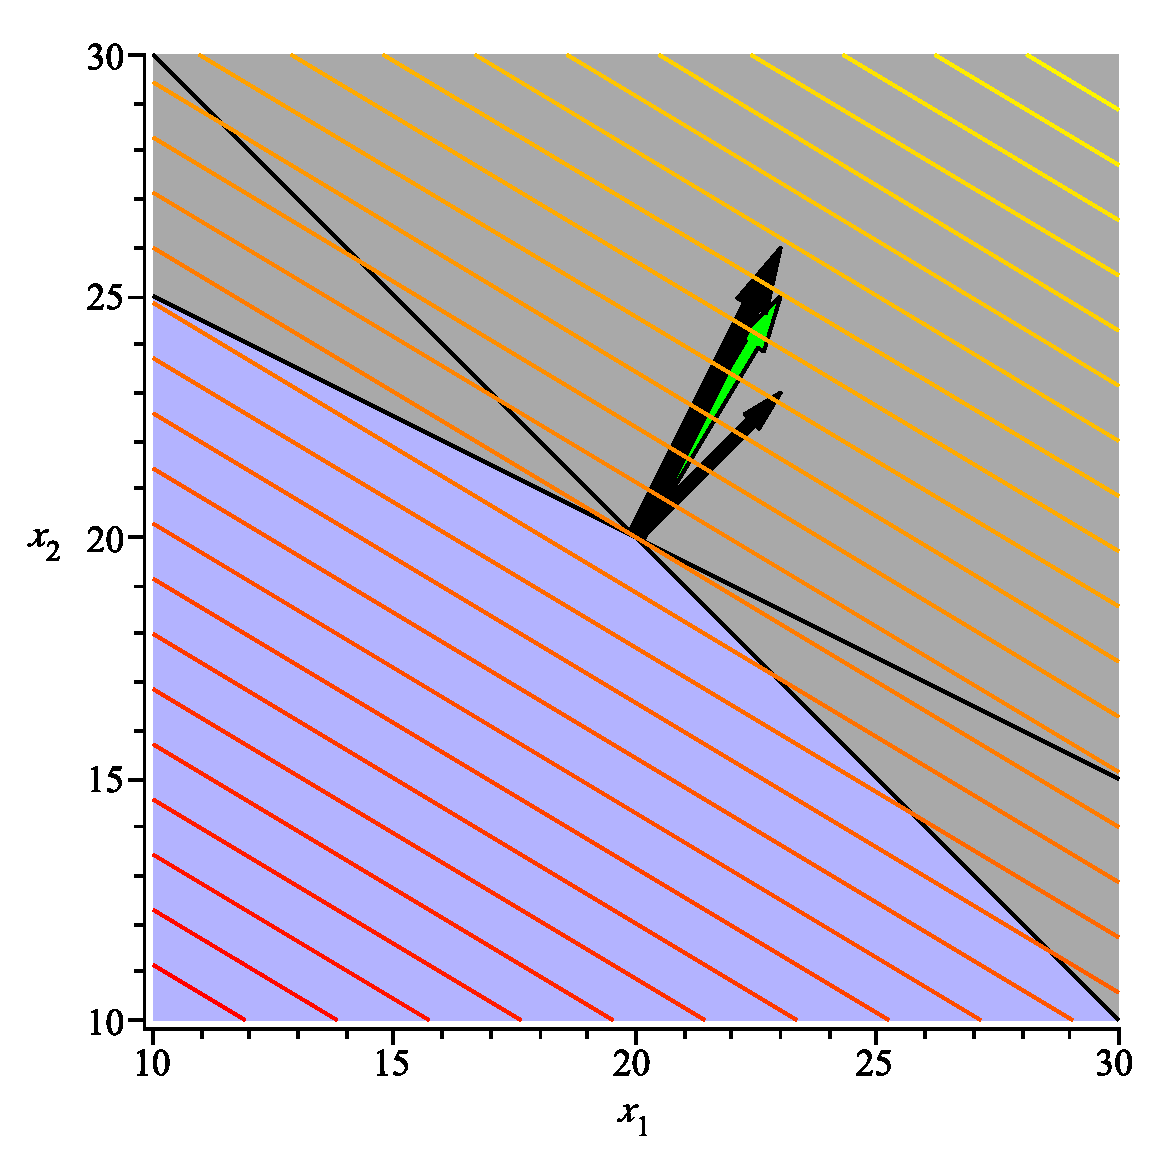
\includegraphics[scale=0.35]{LeatherMakerKKT.pdf}
\caption{This figure illustrates the optimal point of the problem given in Example \ref{ex:KKTSimplex}. Note that at optimality, the objective function gradient is in the dual cone of the binding constraint. That is, it is a positive combination of the gradients of the left-hand-sides of the binding constraints at optimality. The gradient of the objective function is shown in green.}
\label{fig:KKTSimplex}
\end{figure}

We can also verify that the KKT conditions hold for the problem in standard form. Naturally, complementary slackness and primal feasibility hold. To see that dual feasibility holds note that $\mathbf{v} = [0\;\;0\;\;2\;\;1] \geq \mathbf{0}$. Further:
\begin{displaymath}
\begin{bmatrix}2 & 1\end{bmatrix}
\begin{bmatrix} 1 & 2 & 1 & 0\\
1 & 1 & 0 & 1\end{bmatrix} - \begin{bmatrix}
0 & 0 & 2 & 1\end{bmatrix} = \begin{bmatrix} 3 & 5 & 0 & 0\end{bmatrix}
\end{displaymath} 
Here $\begin{bmatrix} 3 & 5 & 0 & 0\end{bmatrix}$ is the objective function coefficient vector for the problem in Standard Form.
\label{ex:KKTSimplex}
\end{example}

\begin{exercise} Use a full simplex tableau to find the values of the Lagrange multipliers (dual variables) at optimality for the problem from Exercise \ref{exer:FindKKT}. Confirm that complementary slackness holds at optimality. Lastly show that dual feasibility holds by showing that the gradient of the objective function ($\mathbf{c}$) is a positive combination of the gradients of the binding constraints at optimality. [Hint: Use the vector $\mathbf{w}$ you should have identified.]
\end{exercise}
